% Created by tikzDevice version 0.6.1 on 2011-08-03 09:51:24
% !TEX encoding = UTF-8 Unicode
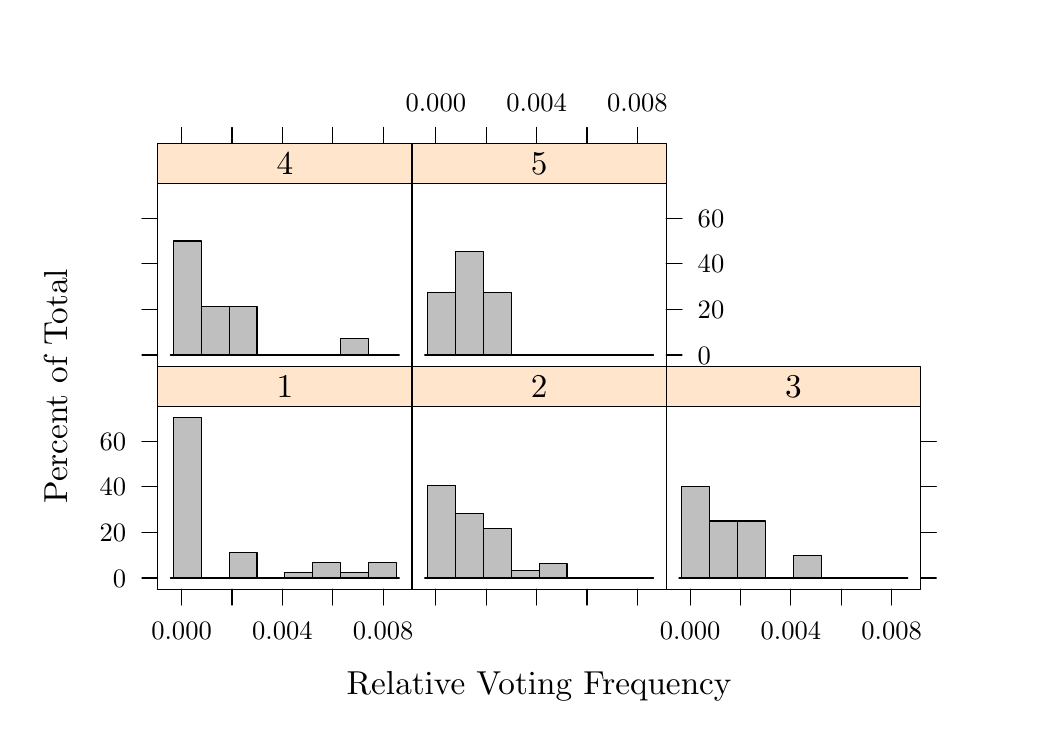
\begin{tikzpicture}[x=1pt,y=1pt]
\definecolor[named]{drawColor}{rgb}{0.00,0.00,0.00}
\definecolor[named]{fillColor}{rgb}{1.00,1.00,1.00}
\fill[color=fillColor,] (0,0) rectangle (361.35,252.94);
\begin{scope}
\path[clip] (  0.00,  0.00) rectangle (361.35,252.94);
\definecolor[named]{fillColor}{rgb}{0.00,0.00,0.00}
\end{scope}
\begin{scope}
\path[clip] (  0.00,  0.00) rectangle (361.35,252.94);
\definecolor[named]{fillColor}{rgb}{0.00,0.00,0.00}

\draw[fill opacity=0.00,draw opacity=0.00,] (  0.00,  0.00) rectangle (361.35,252.94);
\definecolor[named]{drawColor}{rgb}{0.00,0.00,0.00}

\node[color=drawColor,anchor=base,inner sep=0pt, outer sep=0pt, scale=  1.20] at (184.81, 12.04) {Relative Voting Frequency%
};
\end{scope}
\begin{scope}
\path[clip] (  0.00,  0.00) rectangle (361.35,252.94);
\definecolor[named]{fillColor}{rgb}{0.00,0.00,0.00}
\definecolor[named]{drawColor}{rgb}{0.00,0.00,0.00}

\node[rotate= 90.00,color=drawColor,anchor=base,inner sep=0pt, outer sep=0pt, scale=  1.20] at ( 14.29,123.38) {Percent of Total%
};
\end{scope}
\begin{scope}
\path[clip] (  0.00,  0.00) rectangle (361.35,252.94);
\definecolor[named]{fillColor}{rgb}{0.00,0.00,0.00}
\end{scope}
\begin{scope}
\path[clip] (  0.00,  0.00) rectangle (361.35,252.94);
\definecolor[named]{fillColor}{rgb}{0.00,0.00,0.00}
\end{scope}
\begin{scope}
\path[clip] (  0.00,  0.00) rectangle (361.35,252.94);
\definecolor[named]{fillColor}{rgb}{0.00,0.00,0.00}
\end{scope}
\begin{scope}
\path[clip] ( 46.98, 50.02) rectangle (138.86,116.15);
\definecolor[named]{fillColor}{rgb}{0.00,0.00,0.00}
\end{scope}
\begin{scope}
\path[clip] (  0.00,  0.00) rectangle (361.35,252.94);
\definecolor[named]{fillColor}{rgb}{0.00,0.00,0.00}
\end{scope}
\begin{scope}
\path[clip] (  0.00,  0.00) rectangle (361.35,252.94);
\definecolor[named]{fillColor}{rgb}{0.00,0.00,0.00}
\end{scope}
\begin{scope}
\path[clip] (  0.00,  0.00) rectangle (361.35,252.94);
\definecolor[named]{fillColor}{rgb}{0.00,0.00,0.00}
\end{scope}
\begin{scope}
\path[clip] (  0.00,  0.00) rectangle (361.35,252.94);
\definecolor[named]{fillColor}{rgb}{0.00,0.00,0.00}
\definecolor[named]{drawColor}{rgb}{0.00,0.00,0.00}

\draw[color=drawColor,line cap=round,line join=round,fill opacity=0.00,] ( 46.98, 54.08) -- ( 41.29, 54.08);

\draw[color=drawColor,line cap=round,line join=round,fill opacity=0.00,] ( 46.98, 70.54) -- ( 41.29, 70.54);

\draw[color=drawColor,line cap=round,line join=round,fill opacity=0.00,] ( 46.98, 87.01) -- ( 41.29, 87.01);

\draw[color=drawColor,line cap=round,line join=round,fill opacity=0.00,] ( 46.98,103.48) -- ( 41.29,103.48);

\node[color=drawColor,anchor=base east,inner sep=0pt, outer sep=0pt, scale=  0.96] at ( 35.60, 50.77) {0%
};

\node[color=drawColor,anchor=base east,inner sep=0pt, outer sep=0pt, scale=  0.96] at ( 35.60, 67.24) {20%
};

\node[color=drawColor,anchor=base east,inner sep=0pt, outer sep=0pt, scale=  0.96] at ( 35.60, 83.71) {40%
};

\node[color=drawColor,anchor=base east,inner sep=0pt, outer sep=0pt, scale=  0.96] at ( 35.60,100.18) {60%
};
\end{scope}
\begin{scope}
\path[clip] (  0.00,  0.00) rectangle (361.35,252.94);
\definecolor[named]{fillColor}{rgb}{0.00,0.00,0.00}
\end{scope}
\begin{scope}
\path[clip] (  0.00,  0.00) rectangle (361.35,252.94);
\definecolor[named]{fillColor}{rgb}{0.00,0.00,0.00}
\definecolor[named]{drawColor}{rgb}{0.00,0.00,0.00}

\draw[color=drawColor,line cap=round,line join=round,fill opacity=0.00,] ( 55.61, 50.02) -- ( 55.61, 44.32);

\draw[color=drawColor,line cap=round,line join=round,fill opacity=0.00,] ( 73.82, 50.02) -- ( 73.82, 44.32);

\draw[color=drawColor,line cap=round,line join=round,fill opacity=0.00,] ( 92.03, 50.02) -- ( 92.03, 44.32);

\draw[color=drawColor,line cap=round,line join=round,fill opacity=0.00,] (110.24, 50.02) -- (110.24, 44.32);

\draw[color=drawColor,line cap=round,line join=round,fill opacity=0.00,] (128.45, 50.02) -- (128.45, 44.32);

\node[color=drawColor,anchor=base,inner sep=0pt, outer sep=0pt, scale=  0.96] at ( 55.61, 32.02) {0.000%
};

\node[color=drawColor,anchor=base,inner sep=0pt, outer sep=0pt, scale=  0.96] at ( 92.03, 32.02) {0.004%
};

\node[color=drawColor,anchor=base,inner sep=0pt, outer sep=0pt, scale=  0.96] at (128.45, 32.02) {0.008%
};
\end{scope}
\begin{scope}
\path[clip] (  0.00,  0.00) rectangle (361.35,252.94);
\definecolor[named]{fillColor}{rgb}{0.00,0.00,0.00}
\end{scope}
\begin{scope}
\path[clip] ( 46.98, 50.02) rectangle (138.86,116.15);
\definecolor[named]{fillColor}{rgb}{0.00,0.00,0.00}
\definecolor[named]{drawColor}{rgb}{0.00,0.00,0.00}

\draw[color=drawColor,line cap=round,line join=round,fill opacity=0.00,] ( 51.57, 54.08) --
	(134.27, 54.08);
\definecolor[named]{fillColor}{rgb}{0.75,0.75,0.75}

\draw[color=drawColor,line cap=round,line join=round,fill=fillColor,] ( 52.62, 54.08) rectangle ( 62.70,112.09);

\draw[color=drawColor,line cap=round,line join=round,fill=fillColor,] ( 62.70, 54.08) rectangle ( 72.77, 54.08);

\draw[color=drawColor,line cap=round,line join=round,fill=fillColor,] ( 72.77, 54.08) rectangle ( 82.85, 63.43);

\draw[color=drawColor,line cap=round,line join=round,fill=fillColor,] ( 82.85, 54.08) rectangle ( 92.92, 54.08);

\draw[color=drawColor,line cap=round,line join=round,fill=fillColor,] ( 92.92, 54.08) rectangle (103.00, 55.95);

\draw[color=drawColor,line cap=round,line join=round,fill=fillColor,] (103.00, 54.08) rectangle (113.07, 59.69);

\draw[color=drawColor,line cap=round,line join=round,fill=fillColor,] (113.07, 54.08) rectangle (123.15, 55.95);

\draw[color=drawColor,line cap=round,line join=round,fill=fillColor,] (123.15, 54.08) rectangle (133.22, 59.69);
\end{scope}
\begin{scope}
\path[clip] (  0.00,  0.00) rectangle (361.35,252.94);
\definecolor[named]{fillColor}{rgb}{0.00,0.00,0.00}
\end{scope}
\begin{scope}
\path[clip] (  0.00,  0.00) rectangle (361.35,252.94);
\definecolor[named]{fillColor}{rgb}{0.00,0.00,0.00}
\definecolor[named]{drawColor}{rgb}{0.00,0.00,0.00}

\draw[color=drawColor,line cap=round,line join=round,fill opacity=0.00,] ( 46.98, 50.02) rectangle (138.86,116.15);
\end{scope}
\begin{scope}
\path[clip] (  0.00,  0.00) rectangle (361.35,252.94);
\definecolor[named]{fillColor}{rgb}{0.00,0.00,0.00}
\end{scope}
\begin{scope}
\path[clip] (  0.00,  0.00) rectangle (361.35,252.94);
\definecolor[named]{fillColor}{rgb}{0.00,0.00,0.00}
\end{scope}
\begin{scope}
\path[clip] ( 46.98,116.15) rectangle (138.86,130.60);
\definecolor[named]{fillColor}{rgb}{0.00,0.00,0.00}
\definecolor[named]{drawColor}{rgb}{1.00,0.90,0.80}
\definecolor[named]{fillColor}{rgb}{1.00,0.90,0.80}

\draw[color=drawColor,line cap=round,line join=round,fill=fillColor,] ( 46.98,116.15) rectangle (138.86,130.60);
\definecolor[named]{drawColor}{rgb}{0.00,0.00,0.00}

\node[color=drawColor,anchor=base west,inner sep=0pt, outer sep=0pt, scale=  1.20] at ( 89.92,119.25) {1%
};
\end{scope}
\begin{scope}
\path[clip] (  0.00,  0.00) rectangle (361.35,252.94);
\definecolor[named]{fillColor}{rgb}{0.00,0.00,0.00}
\end{scope}
\begin{scope}
\path[clip] (  0.00,  0.00) rectangle (361.35,252.94);
\definecolor[named]{fillColor}{rgb}{0.00,0.00,0.00}
\definecolor[named]{drawColor}{rgb}{0.00,0.00,0.00}

\draw[color=drawColor,line cap=round,line join=round,fill opacity=0.00,] ( 46.98,116.15) rectangle (138.86,130.60);
\end{scope}
\begin{scope}
\path[clip] (  0.00,  0.00) rectangle (361.35,252.94);
\definecolor[named]{fillColor}{rgb}{0.00,0.00,0.00}
\end{scope}
\begin{scope}
\path[clip] (  0.00,  0.00) rectangle (361.35,252.94);
\definecolor[named]{fillColor}{rgb}{0.00,0.00,0.00}
\end{scope}
\begin{scope}
\path[clip] (138.86, 50.02) rectangle (230.75,116.15);
\definecolor[named]{fillColor}{rgb}{0.00,0.00,0.00}
\end{scope}
\begin{scope}
\path[clip] (  0.00,  0.00) rectangle (361.35,252.94);
\definecolor[named]{fillColor}{rgb}{0.00,0.00,0.00}
\end{scope}
\begin{scope}
\path[clip] (  0.00,  0.00) rectangle (361.35,252.94);
\definecolor[named]{fillColor}{rgb}{0.00,0.00,0.00}
\end{scope}
\begin{scope}
\path[clip] (  0.00,  0.00) rectangle (361.35,252.94);
\definecolor[named]{fillColor}{rgb}{0.00,0.00,0.00}
\end{scope}
\begin{scope}
\path[clip] (  0.00,  0.00) rectangle (361.35,252.94);
\definecolor[named]{fillColor}{rgb}{0.00,0.00,0.00}
\end{scope}
\begin{scope}
\path[clip] (  0.00,  0.00) rectangle (361.35,252.94);
\definecolor[named]{fillColor}{rgb}{0.00,0.00,0.00}
\end{scope}
\begin{scope}
\path[clip] (  0.00,  0.00) rectangle (361.35,252.94);
\definecolor[named]{fillColor}{rgb}{0.00,0.00,0.00}
\definecolor[named]{drawColor}{rgb}{0.00,0.00,0.00}

\draw[color=drawColor,line cap=round,line join=round,fill opacity=0.00,] (147.49, 50.02) -- (147.49, 44.32);

\draw[color=drawColor,line cap=round,line join=round,fill opacity=0.00,] (165.70, 50.02) -- (165.70, 44.32);

\draw[color=drawColor,line cap=round,line join=round,fill opacity=0.00,] (183.91, 50.02) -- (183.91, 44.32);

\draw[color=drawColor,line cap=round,line join=round,fill opacity=0.00,] (202.12, 50.02) -- (202.12, 44.32);

\draw[color=drawColor,line cap=round,line join=round,fill opacity=0.00,] (220.33, 50.02) -- (220.33, 44.32);
\end{scope}
\begin{scope}
\path[clip] (  0.00,  0.00) rectangle (361.35,252.94);
\definecolor[named]{fillColor}{rgb}{0.00,0.00,0.00}
\end{scope}
\begin{scope}
\path[clip] (138.86, 50.02) rectangle (230.75,116.15);
\definecolor[named]{fillColor}{rgb}{0.00,0.00,0.00}
\definecolor[named]{drawColor}{rgb}{0.00,0.00,0.00}

\draw[color=drawColor,line cap=round,line join=round,fill opacity=0.00,] (143.46, 54.08) --
	(226.16, 54.08);
\definecolor[named]{fillColor}{rgb}{0.75,0.75,0.75}

\draw[color=drawColor,line cap=round,line join=round,fill=fillColor,] (144.51, 54.08) rectangle (154.58, 87.53);

\draw[color=drawColor,line cap=round,line join=round,fill=fillColor,] (154.58, 54.08) rectangle (164.66, 77.24);

\draw[color=drawColor,line cap=round,line join=round,fill=fillColor,] (164.66, 54.08) rectangle (174.73, 72.09);

\draw[color=drawColor,line cap=round,line join=round,fill=fillColor,] (174.73, 54.08) rectangle (184.81, 56.65);

\draw[color=drawColor,line cap=round,line join=round,fill=fillColor,] (184.81, 54.08) rectangle (194.88, 59.22);

\draw[color=drawColor,line cap=round,line join=round,fill=fillColor,] (194.88, 54.08) rectangle (204.96, 54.08);

\draw[color=drawColor,line cap=round,line join=round,fill=fillColor,] (204.96, 54.08) rectangle (215.03, 54.08);

\draw[color=drawColor,line cap=round,line join=round,fill=fillColor,] (215.03, 54.08) rectangle (225.11, 54.08);
\end{scope}
\begin{scope}
\path[clip] (  0.00,  0.00) rectangle (361.35,252.94);
\definecolor[named]{fillColor}{rgb}{0.00,0.00,0.00}
\end{scope}
\begin{scope}
\path[clip] (  0.00,  0.00) rectangle (361.35,252.94);
\definecolor[named]{fillColor}{rgb}{0.00,0.00,0.00}
\definecolor[named]{drawColor}{rgb}{0.00,0.00,0.00}

\draw[color=drawColor,line cap=round,line join=round,fill opacity=0.00,] (138.86, 50.02) rectangle (230.75,116.15);
\end{scope}
\begin{scope}
\path[clip] (  0.00,  0.00) rectangle (361.35,252.94);
\definecolor[named]{fillColor}{rgb}{0.00,0.00,0.00}
\end{scope}
\begin{scope}
\path[clip] (  0.00,  0.00) rectangle (361.35,252.94);
\definecolor[named]{fillColor}{rgb}{0.00,0.00,0.00}
\end{scope}
\begin{scope}
\path[clip] (138.86,116.15) rectangle (230.75,130.60);
\definecolor[named]{fillColor}{rgb}{0.00,0.00,0.00}
\definecolor[named]{drawColor}{rgb}{1.00,0.90,0.80}
\definecolor[named]{fillColor}{rgb}{1.00,0.90,0.80}

\draw[color=drawColor,line cap=round,line join=round,fill=fillColor,] (138.86,116.15) rectangle (230.75,130.60);
\definecolor[named]{drawColor}{rgb}{0.00,0.00,0.00}

\node[color=drawColor,anchor=base west,inner sep=0pt, outer sep=0pt, scale=  1.20] at (181.81,119.25) {2%
};
\end{scope}
\begin{scope}
\path[clip] (  0.00,  0.00) rectangle (361.35,252.94);
\definecolor[named]{fillColor}{rgb}{0.00,0.00,0.00}
\end{scope}
\begin{scope}
\path[clip] (  0.00,  0.00) rectangle (361.35,252.94);
\definecolor[named]{fillColor}{rgb}{0.00,0.00,0.00}
\definecolor[named]{drawColor}{rgb}{0.00,0.00,0.00}

\draw[color=drawColor,line cap=round,line join=round,fill opacity=0.00,] (138.86,116.15) rectangle (230.75,130.60);
\end{scope}
\begin{scope}
\path[clip] (  0.00,  0.00) rectangle (361.35,252.94);
\definecolor[named]{fillColor}{rgb}{0.00,0.00,0.00}
\end{scope}
\begin{scope}
\path[clip] (  0.00,  0.00) rectangle (361.35,252.94);
\definecolor[named]{fillColor}{rgb}{0.00,0.00,0.00}
\end{scope}
\begin{scope}
\path[clip] (230.75, 50.02) rectangle (322.64,116.15);
\definecolor[named]{fillColor}{rgb}{0.00,0.00,0.00}
\end{scope}
\begin{scope}
\path[clip] (  0.00,  0.00) rectangle (361.35,252.94);
\definecolor[named]{fillColor}{rgb}{0.00,0.00,0.00}
\end{scope}
\begin{scope}
\path[clip] (  0.00,  0.00) rectangle (361.35,252.94);
\definecolor[named]{fillColor}{rgb}{0.00,0.00,0.00}
\end{scope}
\begin{scope}
\path[clip] (  0.00,  0.00) rectangle (361.35,252.94);
\definecolor[named]{fillColor}{rgb}{0.00,0.00,0.00}
\end{scope}
\begin{scope}
\path[clip] (  0.00,  0.00) rectangle (361.35,252.94);
\definecolor[named]{fillColor}{rgb}{0.00,0.00,0.00}
\end{scope}
\begin{scope}
\path[clip] (  0.00,  0.00) rectangle (361.35,252.94);
\definecolor[named]{fillColor}{rgb}{0.00,0.00,0.00}
\end{scope}
\begin{scope}
\path[clip] (  0.00,  0.00) rectangle (361.35,252.94);
\definecolor[named]{fillColor}{rgb}{0.00,0.00,0.00}
\definecolor[named]{drawColor}{rgb}{0.00,0.00,0.00}

\draw[color=drawColor,line cap=round,line join=round,fill opacity=0.00,] (239.38, 50.02) -- (239.38, 44.32);

\draw[color=drawColor,line cap=round,line join=round,fill opacity=0.00,] (257.59, 50.02) -- (257.59, 44.32);

\draw[color=drawColor,line cap=round,line join=round,fill opacity=0.00,] (275.80, 50.02) -- (275.80, 44.32);

\draw[color=drawColor,line cap=round,line join=round,fill opacity=0.00,] (294.01, 50.02) -- (294.01, 44.32);

\draw[color=drawColor,line cap=round,line join=round,fill opacity=0.00,] (312.22, 50.02) -- (312.22, 44.32);

\node[color=drawColor,anchor=base,inner sep=0pt, outer sep=0pt, scale=  0.96] at (239.38, 32.02) {0.000%
};

\node[color=drawColor,anchor=base,inner sep=0pt, outer sep=0pt, scale=  0.96] at (275.80, 32.02) {0.004%
};

\node[color=drawColor,anchor=base,inner sep=0pt, outer sep=0pt, scale=  0.96] at (312.22, 32.02) {0.008%
};

\draw[color=drawColor,line cap=round,line join=round,fill opacity=0.00,] (322.64, 54.08) -- (328.33, 54.08);

\draw[color=drawColor,line cap=round,line join=round,fill opacity=0.00,] (322.64, 70.54) -- (328.33, 70.54);

\draw[color=drawColor,line cap=round,line join=round,fill opacity=0.00,] (322.64, 87.01) -- (328.33, 87.01);

\draw[color=drawColor,line cap=round,line join=round,fill opacity=0.00,] (322.64,103.48) -- (328.33,103.48);
\end{scope}
\begin{scope}
\path[clip] (  0.00,  0.00) rectangle (361.35,252.94);
\definecolor[named]{fillColor}{rgb}{0.00,0.00,0.00}
\end{scope}
\begin{scope}
\path[clip] (230.75, 50.02) rectangle (322.64,116.15);
\definecolor[named]{fillColor}{rgb}{0.00,0.00,0.00}
\definecolor[named]{drawColor}{rgb}{0.00,0.00,0.00}

\draw[color=drawColor,line cap=round,line join=round,fill opacity=0.00,] (235.34, 54.08) --
	(318.04, 54.08);
\definecolor[named]{fillColor}{rgb}{0.75,0.75,0.75}

\draw[color=drawColor,line cap=round,line join=round,fill=fillColor,] (236.39, 54.08) rectangle (246.47, 87.01);

\draw[color=drawColor,line cap=round,line join=round,fill=fillColor,] (246.47, 54.08) rectangle (256.54, 74.66);

\draw[color=drawColor,line cap=round,line join=round,fill=fillColor,] (256.54, 54.08) rectangle (266.62, 74.66);

\draw[color=drawColor,line cap=round,line join=round,fill=fillColor,] (266.62, 54.08) rectangle (276.69, 54.08);

\draw[color=drawColor,line cap=round,line join=round,fill=fillColor,] (276.69, 54.08) rectangle (286.77, 62.31);

\draw[color=drawColor,line cap=round,line join=round,fill=fillColor,] (286.77, 54.08) rectangle (296.84, 54.08);

\draw[color=drawColor,line cap=round,line join=round,fill=fillColor,] (296.84, 54.08) rectangle (306.92, 54.08);

\draw[color=drawColor,line cap=round,line join=round,fill=fillColor,] (306.92, 54.08) rectangle (316.99, 54.08);
\end{scope}
\begin{scope}
\path[clip] (  0.00,  0.00) rectangle (361.35,252.94);
\definecolor[named]{fillColor}{rgb}{0.00,0.00,0.00}
\end{scope}
\begin{scope}
\path[clip] (  0.00,  0.00) rectangle (361.35,252.94);
\definecolor[named]{fillColor}{rgb}{0.00,0.00,0.00}
\definecolor[named]{drawColor}{rgb}{0.00,0.00,0.00}

\draw[color=drawColor,line cap=round,line join=round,fill opacity=0.00,] (230.75, 50.02) rectangle (322.64,116.15);
\end{scope}
\begin{scope}
\path[clip] (  0.00,  0.00) rectangle (361.35,252.94);
\definecolor[named]{fillColor}{rgb}{0.00,0.00,0.00}
\end{scope}
\begin{scope}
\path[clip] (  0.00,  0.00) rectangle (361.35,252.94);
\definecolor[named]{fillColor}{rgb}{0.00,0.00,0.00}
\end{scope}
\begin{scope}
\path[clip] (230.75,116.15) rectangle (322.64,130.60);
\definecolor[named]{fillColor}{rgb}{0.00,0.00,0.00}
\definecolor[named]{drawColor}{rgb}{1.00,0.90,0.80}
\definecolor[named]{fillColor}{rgb}{1.00,0.90,0.80}

\draw[color=drawColor,line cap=round,line join=round,fill=fillColor,] (230.75,116.15) rectangle (322.64,130.60);
\definecolor[named]{drawColor}{rgb}{0.00,0.00,0.00}

\node[color=drawColor,anchor=base west,inner sep=0pt, outer sep=0pt, scale=  1.20] at (273.69,119.25) {3%
};
\end{scope}
\begin{scope}
\path[clip] (  0.00,  0.00) rectangle (361.35,252.94);
\definecolor[named]{fillColor}{rgb}{0.00,0.00,0.00}
\end{scope}
\begin{scope}
\path[clip] (  0.00,  0.00) rectangle (361.35,252.94);
\definecolor[named]{fillColor}{rgb}{0.00,0.00,0.00}
\definecolor[named]{drawColor}{rgb}{0.00,0.00,0.00}

\draw[color=drawColor,line cap=round,line join=round,fill opacity=0.00,] (230.75,116.15) rectangle (322.64,130.60);
\end{scope}
\begin{scope}
\path[clip] (  0.00,  0.00) rectangle (361.35,252.94);
\definecolor[named]{fillColor}{rgb}{0.00,0.00,0.00}
\end{scope}
\begin{scope}
\path[clip] (  0.00,  0.00) rectangle (361.35,252.94);
\definecolor[named]{fillColor}{rgb}{0.00,0.00,0.00}
\end{scope}
\begin{scope}
\path[clip] ( 46.98,130.60) rectangle (138.86,196.74);
\definecolor[named]{fillColor}{rgb}{0.00,0.00,0.00}
\end{scope}
\begin{scope}
\path[clip] (  0.00,  0.00) rectangle (361.35,252.94);
\definecolor[named]{fillColor}{rgb}{0.00,0.00,0.00}
\end{scope}
\begin{scope}
\path[clip] (  0.00,  0.00) rectangle (361.35,252.94);
\definecolor[named]{fillColor}{rgb}{0.00,0.00,0.00}
\definecolor[named]{drawColor}{rgb}{0.00,0.00,0.00}

\draw[color=drawColor,line cap=round,line join=round,fill opacity=0.00,] ( 55.61,211.19) -- ( 55.61,216.88);

\draw[color=drawColor,line cap=round,line join=round,fill opacity=0.00,] ( 73.82,211.19) -- ( 73.82,216.88);

\draw[color=drawColor,line cap=round,line join=round,fill opacity=0.00,] ( 92.03,211.19) -- ( 92.03,216.88);

\draw[color=drawColor,line cap=round,line join=round,fill opacity=0.00,] (110.24,211.19) -- (110.24,216.88);

\draw[color=drawColor,line cap=round,line join=round,fill opacity=0.00,] (128.45,211.19) -- (128.45,216.88);
\end{scope}
\begin{scope}
\path[clip] (  0.00,  0.00) rectangle (361.35,252.94);
\definecolor[named]{fillColor}{rgb}{0.00,0.00,0.00}
\end{scope}
\begin{scope}
\path[clip] (  0.00,  0.00) rectangle (361.35,252.94);
\definecolor[named]{fillColor}{rgb}{0.00,0.00,0.00}
\definecolor[named]{drawColor}{rgb}{0.00,0.00,0.00}

\draw[color=drawColor,line cap=round,line join=round,fill opacity=0.00,] ( 46.98,134.67) -- ( 41.29,134.67);

\draw[color=drawColor,line cap=round,line join=round,fill opacity=0.00,] ( 46.98,151.13) -- ( 41.29,151.13);

\draw[color=drawColor,line cap=round,line join=round,fill opacity=0.00,] ( 46.98,167.60) -- ( 41.29,167.60);

\draw[color=drawColor,line cap=round,line join=round,fill opacity=0.00,] ( 46.98,184.07) -- ( 41.29,184.07);
\end{scope}
\begin{scope}
\path[clip] (  0.00,  0.00) rectangle (361.35,252.94);
\definecolor[named]{fillColor}{rgb}{0.00,0.00,0.00}
\end{scope}
\begin{scope}
\path[clip] (  0.00,  0.00) rectangle (361.35,252.94);
\definecolor[named]{fillColor}{rgb}{0.00,0.00,0.00}
\end{scope}
\begin{scope}
\path[clip] (  0.00,  0.00) rectangle (361.35,252.94);
\definecolor[named]{fillColor}{rgb}{0.00,0.00,0.00}
\end{scope}
\begin{scope}
\path[clip] ( 46.98,130.60) rectangle (138.86,196.74);
\definecolor[named]{fillColor}{rgb}{0.00,0.00,0.00}
\definecolor[named]{drawColor}{rgb}{0.00,0.00,0.00}

\draw[color=drawColor,line cap=round,line join=round,fill opacity=0.00,] ( 51.57,134.67) --
	(134.27,134.67);
\definecolor[named]{fillColor}{rgb}{0.75,0.75,0.75}

\draw[color=drawColor,line cap=round,line join=round,fill=fillColor,] ( 52.62,134.67) rectangle ( 62.70,175.84);

\draw[color=drawColor,line cap=round,line join=round,fill=fillColor,] ( 62.70,134.67) rectangle ( 72.77,152.31);

\draw[color=drawColor,line cap=round,line join=round,fill=fillColor,] ( 72.77,134.67) rectangle ( 82.85,152.31);

\draw[color=drawColor,line cap=round,line join=round,fill=fillColor,] ( 82.85,134.67) rectangle ( 92.92,134.67);

\draw[color=drawColor,line cap=round,line join=round,fill=fillColor,] ( 92.92,134.67) rectangle (103.00,134.67);

\draw[color=drawColor,line cap=round,line join=round,fill=fillColor,] (103.00,134.67) rectangle (113.07,134.67);

\draw[color=drawColor,line cap=round,line join=round,fill=fillColor,] (113.07,134.67) rectangle (123.15,140.55);

\draw[color=drawColor,line cap=round,line join=round,fill=fillColor,] (123.15,134.67) rectangle (133.22,134.67);
\end{scope}
\begin{scope}
\path[clip] (  0.00,  0.00) rectangle (361.35,252.94);
\definecolor[named]{fillColor}{rgb}{0.00,0.00,0.00}
\end{scope}
\begin{scope}
\path[clip] (  0.00,  0.00) rectangle (361.35,252.94);
\definecolor[named]{fillColor}{rgb}{0.00,0.00,0.00}
\definecolor[named]{drawColor}{rgb}{0.00,0.00,0.00}

\draw[color=drawColor,line cap=round,line join=round,fill opacity=0.00,] ( 46.98,130.60) rectangle (138.86,196.74);
\end{scope}
\begin{scope}
\path[clip] (  0.00,  0.00) rectangle (361.35,252.94);
\definecolor[named]{fillColor}{rgb}{0.00,0.00,0.00}
\end{scope}
\begin{scope}
\path[clip] (  0.00,  0.00) rectangle (361.35,252.94);
\definecolor[named]{fillColor}{rgb}{0.00,0.00,0.00}
\end{scope}
\begin{scope}
\path[clip] ( 46.98,196.74) rectangle (138.86,211.19);
\definecolor[named]{fillColor}{rgb}{0.00,0.00,0.00}
\definecolor[named]{drawColor}{rgb}{1.00,0.90,0.80}
\definecolor[named]{fillColor}{rgb}{1.00,0.90,0.80}

\draw[color=drawColor,line cap=round,line join=round,fill=fillColor,] ( 46.98,196.74) rectangle (138.86,211.19);
\definecolor[named]{drawColor}{rgb}{0.00,0.00,0.00}

\node[color=drawColor,anchor=base west,inner sep=0pt, outer sep=0pt, scale=  1.20] at ( 89.92,199.83) {4%
};
\end{scope}
\begin{scope}
\path[clip] (  0.00,  0.00) rectangle (361.35,252.94);
\definecolor[named]{fillColor}{rgb}{0.00,0.00,0.00}
\end{scope}
\begin{scope}
\path[clip] (  0.00,  0.00) rectangle (361.35,252.94);
\definecolor[named]{fillColor}{rgb}{0.00,0.00,0.00}
\definecolor[named]{drawColor}{rgb}{0.00,0.00,0.00}

\draw[color=drawColor,line cap=round,line join=round,fill opacity=0.00,] ( 46.98,196.74) rectangle (138.86,211.19);
\end{scope}
\begin{scope}
\path[clip] (  0.00,  0.00) rectangle (361.35,252.94);
\definecolor[named]{fillColor}{rgb}{0.00,0.00,0.00}
\end{scope}
\begin{scope}
\path[clip] (  0.00,  0.00) rectangle (361.35,252.94);
\definecolor[named]{fillColor}{rgb}{0.00,0.00,0.00}
\end{scope}
\begin{scope}
\path[clip] (138.86,130.60) rectangle (230.75,196.74);
\definecolor[named]{fillColor}{rgb}{0.00,0.00,0.00}
\end{scope}
\begin{scope}
\path[clip] (  0.00,  0.00) rectangle (361.35,252.94);
\definecolor[named]{fillColor}{rgb}{0.00,0.00,0.00}
\end{scope}
\begin{scope}
\path[clip] (  0.00,  0.00) rectangle (361.35,252.94);
\definecolor[named]{fillColor}{rgb}{0.00,0.00,0.00}
\definecolor[named]{drawColor}{rgb}{0.00,0.00,0.00}

\draw[color=drawColor,line cap=round,line join=round,fill opacity=0.00,] (147.49,211.19) -- (147.49,216.88);

\draw[color=drawColor,line cap=round,line join=round,fill opacity=0.00,] (165.70,211.19) -- (165.70,216.88);

\draw[color=drawColor,line cap=round,line join=round,fill opacity=0.00,] (183.91,211.19) -- (183.91,216.88);

\draw[color=drawColor,line cap=round,line join=round,fill opacity=0.00,] (202.12,211.19) -- (202.12,216.88);

\draw[color=drawColor,line cap=round,line join=round,fill opacity=0.00,] (220.33,211.19) -- (220.33,216.88);

\node[color=drawColor,anchor=base,inner sep=0pt, outer sep=0pt, scale=  0.96] at (147.49,222.58) {0.000%
};

\node[color=drawColor,anchor=base,inner sep=0pt, outer sep=0pt, scale=  0.96] at (183.91,222.58) {0.004%
};

\node[color=drawColor,anchor=base,inner sep=0pt, outer sep=0pt, scale=  0.96] at (220.33,222.58) {0.008%
};
\end{scope}
\begin{scope}
\path[clip] (  0.00,  0.00) rectangle (361.35,252.94);
\definecolor[named]{fillColor}{rgb}{0.00,0.00,0.00}
\end{scope}
\begin{scope}
\path[clip] (  0.00,  0.00) rectangle (361.35,252.94);
\definecolor[named]{fillColor}{rgb}{0.00,0.00,0.00}
\end{scope}
\begin{scope}
\path[clip] (  0.00,  0.00) rectangle (361.35,252.94);
\definecolor[named]{fillColor}{rgb}{0.00,0.00,0.00}
\end{scope}
\begin{scope}
\path[clip] (  0.00,  0.00) rectangle (361.35,252.94);
\definecolor[named]{fillColor}{rgb}{0.00,0.00,0.00}
\definecolor[named]{drawColor}{rgb}{0.00,0.00,0.00}

\draw[color=drawColor,line cap=round,line join=round,fill opacity=0.00,] (230.75,134.67) -- (236.44,134.67);

\draw[color=drawColor,line cap=round,line join=round,fill opacity=0.00,] (230.75,151.13) -- (236.44,151.13);

\draw[color=drawColor,line cap=round,line join=round,fill opacity=0.00,] (230.75,167.60) -- (236.44,167.60);

\draw[color=drawColor,line cap=round,line join=round,fill opacity=0.00,] (230.75,184.07) -- (236.44,184.07);

\node[color=drawColor,anchor=base west,inner sep=0pt, outer sep=0pt, scale=  0.96] at (242.13,131.36) {0%
};

\node[color=drawColor,anchor=base west,inner sep=0pt, outer sep=0pt, scale=  0.96] at (242.13,147.83) {20%
};

\node[color=drawColor,anchor=base west,inner sep=0pt, outer sep=0pt, scale=  0.96] at (242.13,164.30) {40%
};

\node[color=drawColor,anchor=base west,inner sep=0pt, outer sep=0pt, scale=  0.96] at (242.13,180.76) {60%
};
\end{scope}
\begin{scope}
\path[clip] (  0.00,  0.00) rectangle (361.35,252.94);
\definecolor[named]{fillColor}{rgb}{0.00,0.00,0.00}
\end{scope}
\begin{scope}
\path[clip] (138.86,130.60) rectangle (230.75,196.74);
\definecolor[named]{fillColor}{rgb}{0.00,0.00,0.00}
\definecolor[named]{drawColor}{rgb}{0.00,0.00,0.00}

\draw[color=drawColor,line cap=round,line join=round,fill opacity=0.00,] (143.46,134.67) --
	(226.16,134.67);
\definecolor[named]{fillColor}{rgb}{0.75,0.75,0.75}

\draw[color=drawColor,line cap=round,line join=round,fill=fillColor,] (144.51,134.67) rectangle (154.58,157.12);

\draw[color=drawColor,line cap=round,line join=round,fill=fillColor,] (154.58,134.67) rectangle (164.66,172.09);

\draw[color=drawColor,line cap=round,line join=round,fill=fillColor,] (164.66,134.67) rectangle (174.73,157.12);

\draw[color=drawColor,line cap=round,line join=round,fill=fillColor,] (174.73,134.67) rectangle (184.81,134.67);

\draw[color=drawColor,line cap=round,line join=round,fill=fillColor,] (184.81,134.67) rectangle (194.88,134.67);

\draw[color=drawColor,line cap=round,line join=round,fill=fillColor,] (194.88,134.67) rectangle (204.96,134.67);

\draw[color=drawColor,line cap=round,line join=round,fill=fillColor,] (204.96,134.67) rectangle (215.03,134.67);

\draw[color=drawColor,line cap=round,line join=round,fill=fillColor,] (215.03,134.67) rectangle (225.11,134.67);
\end{scope}
\begin{scope}
\path[clip] (  0.00,  0.00) rectangle (361.35,252.94);
\definecolor[named]{fillColor}{rgb}{0.00,0.00,0.00}
\end{scope}
\begin{scope}
\path[clip] (  0.00,  0.00) rectangle (361.35,252.94);
\definecolor[named]{fillColor}{rgb}{0.00,0.00,0.00}
\definecolor[named]{drawColor}{rgb}{0.00,0.00,0.00}

\draw[color=drawColor,line cap=round,line join=round,fill opacity=0.00,] (138.86,130.60) rectangle (230.75,196.74);
\end{scope}
\begin{scope}
\path[clip] (  0.00,  0.00) rectangle (361.35,252.94);
\definecolor[named]{fillColor}{rgb}{0.00,0.00,0.00}
\end{scope}
\begin{scope}
\path[clip] (  0.00,  0.00) rectangle (361.35,252.94);
\definecolor[named]{fillColor}{rgb}{0.00,0.00,0.00}
\end{scope}
\begin{scope}
\path[clip] (138.86,196.74) rectangle (230.75,211.19);
\definecolor[named]{fillColor}{rgb}{0.00,0.00,0.00}
\definecolor[named]{drawColor}{rgb}{1.00,0.90,0.80}
\definecolor[named]{fillColor}{rgb}{1.00,0.90,0.80}

\draw[color=drawColor,line cap=round,line join=round,fill=fillColor,] (138.86,196.74) rectangle (230.75,211.19);
\definecolor[named]{drawColor}{rgb}{0.00,0.00,0.00}

\node[color=drawColor,anchor=base west,inner sep=0pt, outer sep=0pt, scale=  1.20] at (181.81,199.83) {5%
};
\end{scope}
\begin{scope}
\path[clip] (  0.00,  0.00) rectangle (361.35,252.94);
\definecolor[named]{fillColor}{rgb}{0.00,0.00,0.00}
\end{scope}
\begin{scope}
\path[clip] (  0.00,  0.00) rectangle (361.35,252.94);
\definecolor[named]{fillColor}{rgb}{0.00,0.00,0.00}
\definecolor[named]{drawColor}{rgb}{0.00,0.00,0.00}

\draw[color=drawColor,line cap=round,line join=round,fill opacity=0.00,] (138.86,196.74) rectangle (230.75,211.19);
\end{scope}
\begin{scope}
\path[clip] (  0.00,  0.00) rectangle (361.35,252.94);
\definecolor[named]{fillColor}{rgb}{0.00,0.00,0.00}
\end{scope}
\begin{scope}
\path[clip] (  0.00,  0.00) rectangle (361.35,252.94);
\definecolor[named]{fillColor}{rgb}{0.00,0.00,0.00}
\end{scope}
\begin{scope}
\path[clip] (  0.00,  0.00) rectangle (361.35,252.94);
\definecolor[named]{fillColor}{rgb}{0.00,0.00,0.00}
\end{scope}
\begin{scope}
\path[clip] (  0.00,  0.00) rectangle (361.35,252.94);
\definecolor[named]{fillColor}{rgb}{0.00,0.00,0.00}
\end{scope}
\end{tikzpicture}
